\documentclass[usletter]{article}
\usepackage{graphicx}
\usepackage{amsfonts}
\usepackage{amsthm}
\usepackage{amsmath}
\usepackage{amssymb}
\usepackage{hyperref}
\hypersetup{
    colorlinks=true,
    linkcolor=blue,
    filecolor=magenta,      
    urlcolor=cyan,
}
\usepackage{scribe}
\usepackage[margin=1.5in]{geometry}

\begin{document}

	
\makeheader{Sanket Kanjalkar, Yunqi Li}                              % your name
           {October 09, 2019}                          % lecture date
           {11}                                       % lecture number
           {Fully Homomorphic Encryption I}  % lecture title

\newcommand{\floor}[1]{\left\lfloor #1 \right\rfloor}
\newcommand{\ceil}[1]{\left\lceil #1 \right\rceil}

Informally, a cryptosystem that supports arbitrary computation on ciphertexts is known as fully homomorphic encryption (FHE)\cite{wiki}. Throughout the course, we have studied encryption schemes for the purpose of information transfer from other party to the other. However, if we were to compute on data using our traditional encryption schemes, it would require that data must be decrypted before it can be analyzed or manipulated. It would be great if we can outsource the computation while keeping the data encrypted. That is, it should be possible to compute a known function on encrupted data without having access to the secret key. 

Such a FHE scheme can be used for privacy-preserving outsourced storage and computation. In today's lecture, we will see what is fully homomorphic encryption (FHE) scheme and how to build a FHE scheme achieving homomorphism. We will also look at intuitive ways to construct FHE for addition and multiplication.

\begin{fact}
LWE is the only way we know to do an fully homomorphic encryption as of Oct 2019. 
\end{fact}
           
\section{Recap}

Before stepping into how to build LWE-based FHE schemes, let's briefly recap how to build private and public encryption scheme with LWE problem.
Desisional LWE is the problem where given a matrix $A_{n,m}$, and a corresponding LWE vector result $b_m$, determining whether or not these 
and results vector of some instance of an LWE problem OR whether the vector $b_m$ was simply 
drawn from sampling values uniformly randomly from $Z^{m}_{q}$. 
\begin{definition}
\textbf{\textit{Decisional $LWE{n,m,q,\mathcal{X}}$}} : For all non-uniform probabilistic polynomial time adversary $\mathcal{A}$
$$|\underset{\substack{
\pmb{s}\leftarrow \mathbb{Z}_q^{n\times1}\\
\pmb{A}\leftarrow\mathbb{Z}_q^{n\times m}\\
\pmb{e}\leftarrow \mathcal{X}^m}}{Pr}
[\mathcal{A}(\pmb{A},\pmb{s}^T\pmb{A}+\pmb{e}^T)=1]
-\underset{\substack{\pmb{A}\leftarrow\mathbb{Z}_q^{n\times m}\\
\pmb{b}\leftarrow\mathbb{Z}_q^m}}{Pr} 
[\mathcal{A}(\pmb{A},\pmb{b})=1]|=negl(n)$$
where $q$ is a prime within $O(2^n)$, $m=O(n\log q)$ and norm $\parallel \pmb{e}\parallel=\omega(\log n)$. Where $\omega(f(n))$ means that 
$e$ should be greater than $f(n)$ assymptotically.
\end{definition}

Next we revise the secret key encryption (SKE) built with LWE which has $m=1$:

$$KeyGen(1^n): \pmb{s}\leftarrow\mathbb{Z}_q^n$$
$$\underset{\substack{
\pmb{s}\leftarrow \mathbb{Z}_q^{n\times1}\\
\pmb{a}\leftarrow\mathbb{Z}_q^{n\times 1}\\
\pmb{e}\leftarrow \mathcal{X}}}{Enc}(\pmb{s},\mu\in\{0,1\}): (\pmb{a}, (b = \pmb{s}^T\pmb{a}+e+\mu\lfloor\frac{q}{2}\rfloor)\mod q)$$


$$Dec(\pmb{s},\pmb{a},b): b-\langle\pmb{s}^T,\pmb{a}\rangle=(e+\mu\lfloor\frac{q}{2}\rfloor) \mod q =   
  \begin{cases}
    (0 + 1)* & \text{if $P = \mathit{NP}$} \\
    \emptyset & \text{otherwise}
  \end{cases}$$

LWE can also be used to build public key encryption (PKE):
\begin{itemize}
\item \item $KeyGen(1^n): (sk=\pmb{s},pk=(\pmb{A}, \pmb{b}^T=\pmb{s}^T\pmb{A}+\pmb{e}^T))$
\begin{itemize}
\item[*]  $\pmb{s}\leftarrow\mathbb{Z}_q^n$
\item[*] $\pmb{A}\leftarrow\mathbb{Z}_q^{n\times m}$
\item[*] $\pmb{e}\leftarrow\mathcal{X}^m$
\end{itemize}

\item $Enc(pk,\mu\in\{0,1\}): (\pmb{c_1}=\pmb{A}\pmb{r}, c_2=(\pmb{b}^T\pmb{r}+\mu\lfloor\frac{q}{2}\rfloor)\mod q)$
\begin{itemize}
\item[*]  $\pmb{r}\longleftarrow\{0,1\}^m$
\end{itemize}

\item $Dec(sk,(\pmb{c_1},c_2)): c_2-\pmb{s}^T\pmb{c_1}=\pmb{e}^T\pmb{r}+\mu\lfloor\frac{q}{2}\rfloor$
\end{itemize}


\section{Fully Homomorphic Encryption (FHE)}

Let us consider the scenario shown in \ref{com}. A client has a secret value $x$. The client wants the server do some computation on $x$ without revealing what $x$ is. Firstly, a ciphertext $ct=Enc(x)$ is sent to the server along with the desired function $f$. Then the server could compute a new ciphertext $ct^*=Enc(f(x))$ by evaluating $x$ on another function $g$ which is publicly computable from $f$. After receiving $ct^*$ from the server, the client can use its secret key $sk$ to get the desired result of $f(x)$.

\begin{figure}[!htbp]
\begin{center}
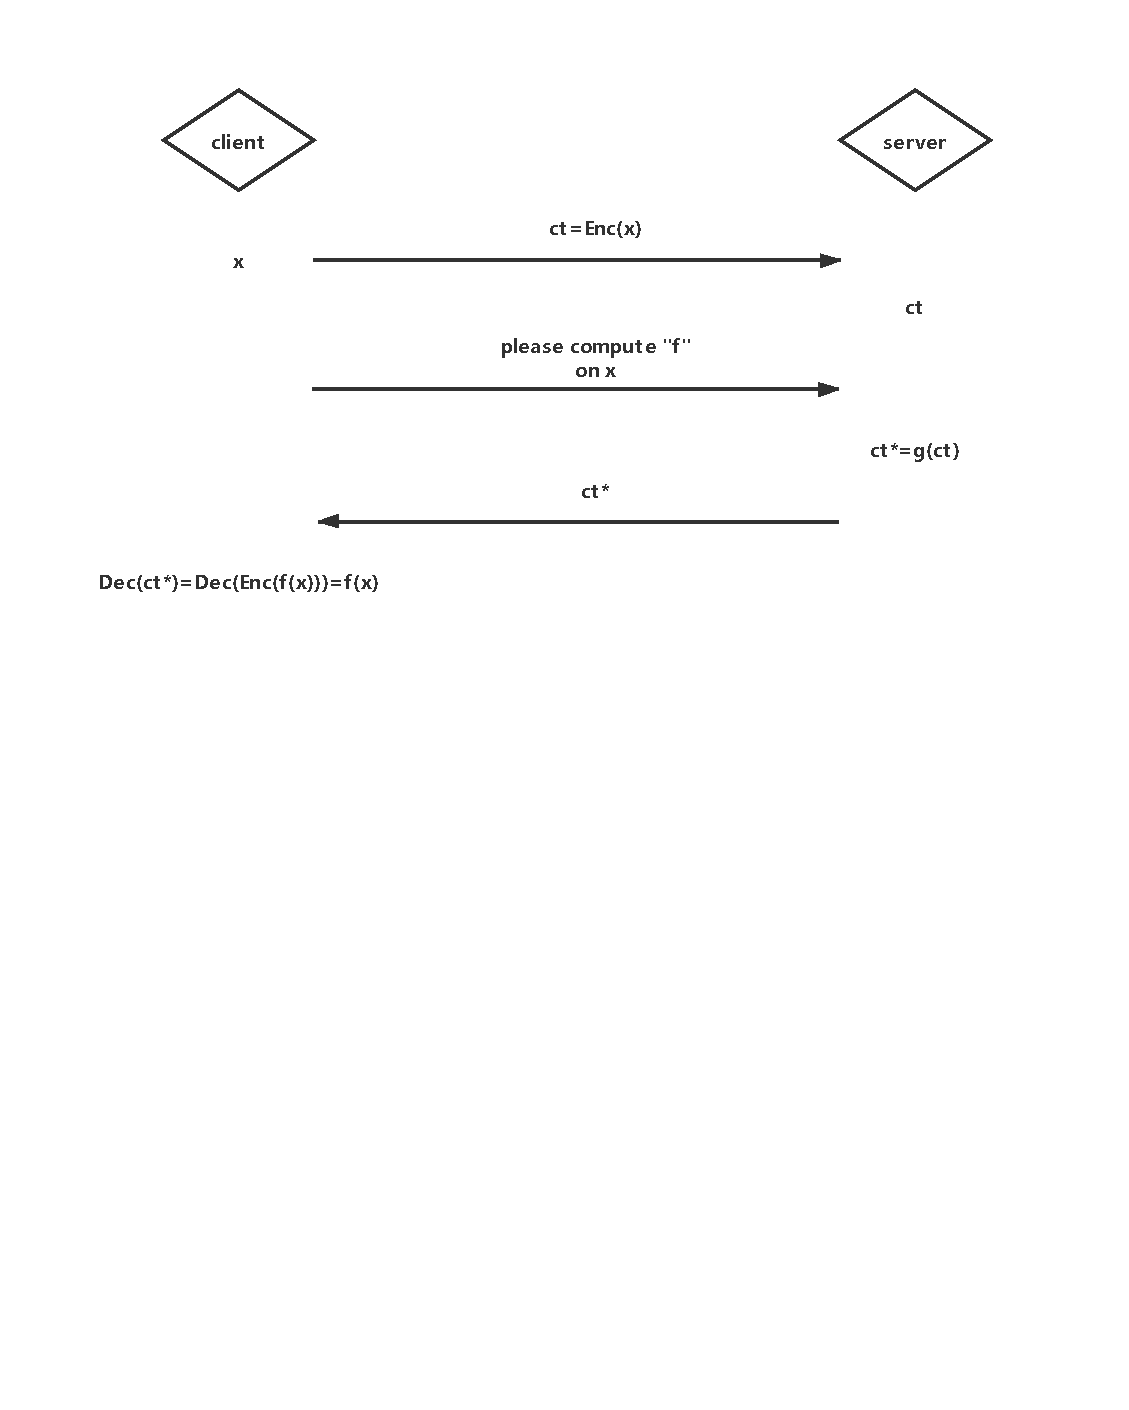
\includegraphics[width=0.9\textwidth]{client-server.pdf}
\end{center}
\caption{Outsourced Computation}
\label{fig:com}
\end{figure}

A homomorphic encryption  can be used for privacy-preserving outsourced storage and computation. It allows operations and analysis on encrypted data without revealing the original one, which removes the privacy barriers in several real-life applications.

\begin{definition} Let $\mathcal{C}$ be a class of circuits where for each $f\in\mathcal{C}$, $f:\{0,1\}^n \rightarrow \{0,1\}$. An encryption scheme $(KeyGen, Enc, Dec, Eval)$ is \textbf{$\mathcal{C}$-homomorphic} if $\forall f\in \mathcal{C}$, all ciphertexts $ct_1, \dots, ct_n$, $Eval(f, ct_1,\dots,ct_n)=ct^*$ such that if  $\forall i$, $\exists m_i, r_i$ s.t. $ct_i=Enc(m_i;r_i)$, then $Dec_{sk}(ct^*)=f(m_1,\dots,m_n)$ and the scheme is IND-CPA secure.
\end{definition}
At a high level, given ciphertexts $ct_1,\dots,ct_n$ that encrypt $m_1,\dots,m_n$, FHE should allow anyone to output a ciphertext  $ct^*$ that encrypts $f(m_1,\dots,m_n)$ for any desired function $f$ by evaluating another function $g$ which is publicly computable from $f$. Thus, the key holder could use the secret key $sk$ to decrypt $ct^*$ and get the result of $f(m_1,\dots,m_n)$. 

Note that each function $f:\{0,1\}^n\rightarrow\{0,1\}^k$ can be split into $f_1,\dots,f_k$ where $\forall i$, $f_i:\{0,1\}^n\rightarrow\{0,1\}$ and also we can generalized the definition by regulating the input length of circuits in $\mathcal{C}$ from $n$ to $poly(n)$.

\section{Construction of Fully Homomorphic Encryption:}
As described previousy, FHE is an ecryption scheme(Gen, Enc, Dec) 
with an additional algorithm called Eval. In particular, we want to construct 
such a Eval namely for two operations, Addition and Multiplication. Constructing 
such a FHE scheme which must work for \textbf{all} functions $f$ might seem like daunting task, 
but can use the following fact to ease our task.
\begin{fact}
It turns out that all functions can be expressed by arithematic circuits consisting
of only addition and multiplication gates. Therefore, we only to implement our FHE operations for 
addition and Multiplication. We can recursively compute every gate  in the Arthematic circuit 
homomorphically to get the output of the function. 
\end{fact}

\begin{definition}
An arithmetic circuit over a field $Z_q$ is a directed
acyclic graph whose vertices are called gates. Gates of incoming degree 0 are inputs to
the circuit. All other gates are labelled $+$ or $x$. 
\end{definition}
We usually consider Arithematic circuits of fan-in 2 circuits, in which 
case all of the + and × gates have in-degree 2.

\begin{remark}
Even though Fully Homomorphic encryption scheme is our actual goal, in practice we also consider 
a simplification leveled fully homomorphic encryption scheme. Leveled FHE does not allow us to 
compute aribritary functions $f$ but only functions with apriory known depth $d$. Informally, when 
we already know what is the most complex(in terms of depth of the arithematic circuit) and use that 
in the construction of our FHE
\end{remark}

Let us try to the simplest possible way to build a FHE for the addition operation. 
For simplicity, let us consider that we want to single bit numbers 
and output a single bit number. This is equivalent to implementing the XOR operation. 

\section{FHE: Addition operation}

	Consider a encryption of message $\mu_1$ under the public key ($s^{T}A + e^{T}$, $A$). We call 
$s^{T}A + e^{T}$ as $b$. One intuitive naive way to implementing addition might be addition of 
ciphertexts

$$c_1 = ( Ar_1, br_1 + \mu_1\floor{\frac{q}{2}} )$$
$$c_1 = ( Ar_2, br_2 + \mu_2\floor{\frac{q}{2}} )$$
$$c_{add} = c_1 + c_2 = ( A(r_1 + r_2), b(r_1 +r_2) + (\mu_1 + \mu_2)\floor{\frac{q}{2}} )$$

It is possible to extend this to multi-bit XOR outputs by simply repeating 
the circuit multiple times. However, it would only help in computing XOR for two $k$ bit numbers. 
Let us try to decrypt the ciphertext $c_{add}$ and check what it decrypts to:

% Copy the decryption equation here.


So applying the decryption algorithm we get $\mu_1$ + $\mu_2$ given the total error
is small ($|e_1 +e_2| \leq q/4$). The important observation to note here is to perform addition on 
two ciphertexts we need to assume hardness of LWE for stronger security parameters. 
Therefore, if we want to perform $l$ addition operations, we would have to keep our $max(e_i) \leq \floor{\frac{q}{2}}/l$.   

\begin{corollary}
To compute addition of $k$ bit numbers $\mu_1$ and $\mu_2$ we must change our 
encryption scheme to the where the factor which is multiplied to the plaintext should be $\frac{q}{2^(k+1)}$. 

$$c_1 = ( Ar_1, br_1 + \mu_1\floor{\frac{q}{2^{k+1}}} )$$
$$c_1 = ( Ar_2, br_2 + \mu_2\floor{\frac{q}{2^{k+1}}} )$$
$$c_{add} = c_1 + c_2 = ( A(r_1 + r_2), b(r_1 +r_2) + (\mu_1 + \mu_2)\floor{\frac{q}{2^{k+1}}} )$$

On the basis of the similar argument described above, the error of the equations for 1 addition be 
constrained by $e_i \leq \frac{q}{2^{k+1}}$.
\end{corollary}
\begin{remark}
It is also possible to implement a similar addition for the private key ecryption part scheme 
using LWE. That is, adding two ciphertexts $c_1$ and $c_2$ corresponding to $\mu_1$ and $\mu_2$
would also result in encryption of message $\mu_1 + \mu_2$.
\end{remark}

\begin{remark}
A natural question which arises from the above discussion is about the similarility XOR operation 
and addition operations.   
\end{remark}

\section{Towards FHE multiplication}

\begin{theorem}
Statement here 
\end{theorem}

\begin{lemma}
Statement here
\end{lemma}

\begin{corollary}
Statement here
\end{corollary}

\begin{proposition}
Statement here
\end{proposition}

\begin{fact}
Statement here
\end{fact}

\begin{claim}
Statement here
\end{claim}

\begin{definition}
Statement here
\end{definition}

\begin{example}
Statement here
\end{example}

\begin{assumption}
Statement here
\end{assumption}

\begin{remark}
Statement here
\end{remark}

\begin{conjecture}
Statement here
\end{conjecture}

\begin{openproblem}
Statement here
\end{openproblem}

\begin{problem}
Statement here
\end{problem}


\noindent
\begin{align}
a = a_1+a_2+\cdots+a_n.
\end{align}
\noindent
For proofs, use the provided {\tt proof} environment,
illustrated below.

\begin{proof}
Proof goes here.
\end{proof}

\section*{Acknowledgement}
These scribe notes were prepared by editing a light modification of the template designed by Alexander Sherstov.
%retain this acknowledgement in all scribe notes.

\bibliographystyle{abbrv}
\bibliography{template}

\end{document}
